\documentclass{article}

\usepackage{hyperref}

\usepackage{epstopdf}
\usepackage{amsmath}
\usepackage{amssymb}
\usepackage{subfig}
%\usepackage{multirow}
\usepackage[utf8]{inputenc}
\usepackage[T1]{fontenc}
\usepackage{standalone}
\usepackage{tikz}
\usepackage{tabularx}

\graphicspath{{img/}}
\DeclareGraphicsExtensions{.pdf,.png,.jpg} %For pdflatex

\begin{document}

\newcommand{\ww}{0.32}

\begin{figure}
%
\captionsetup[subfloat]{position=bottom,labelformat=empty} %można usunąć labelformat wówczas będzie label a), b), c) plus "opis"
\subfloat[opis]{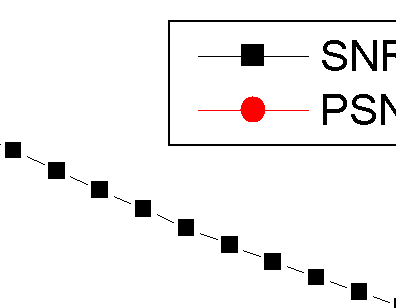
\includegraphics[width=\ww\linewidth]{nazwapliku}}
\hfill%
\subfloat[opis]{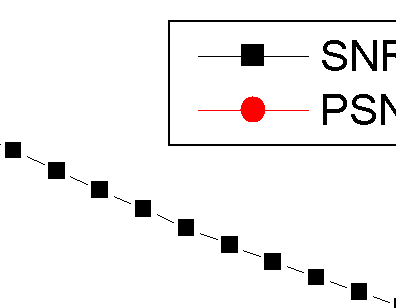
\includegraphics[width=\ww\linewidth]{nazwapliku}}
\hfill% wypełnenie
\subfloat[opis]{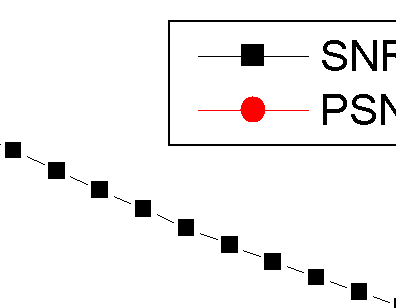
\includegraphics[width=\ww\linewidth]{nazwapliku}}\\ %nowa linia
\subfloat[opis]{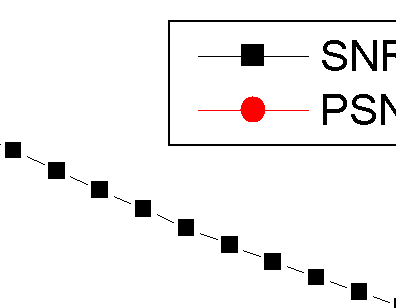
\includegraphics[width=\ww\linewidth]{nazwapliku}}
\hfill%
\subfloat[opis]{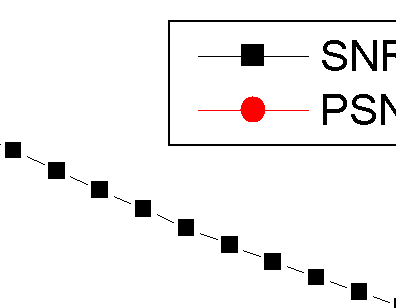
\includegraphics[width=\ww\linewidth]{nazwapliku}}
\hfill%
\subfloat[opis]{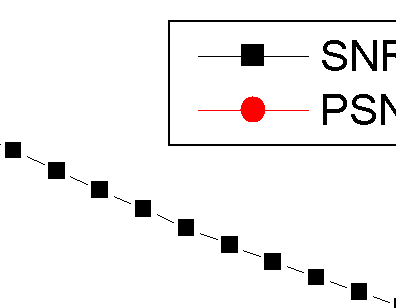
\includegraphics[width=\ww\linewidth]{nazwapliku}}
\caption{Podpis całej ilustracji} %
\label{fig:fig1}
\end{figure}


\renewcommand{\ww}{.16}
\begin{figure}
%
\captionsetup[subfloat]{position=bottom,labelformat=empty} %można usunąć labelformat wówczas będzie label a), b), c) plus "opis"
\subfloat[opis]{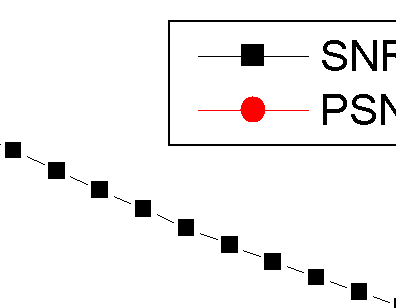
\includegraphics[width=\ww\linewidth]{nazwapliku}}
\hfill%
\subfloat[opis]{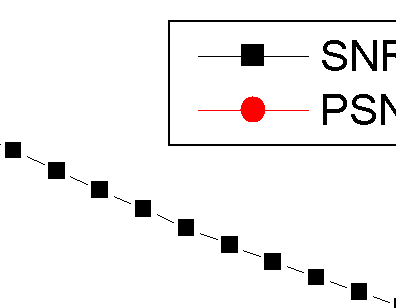
\includegraphics[width=\ww\linewidth]{nazwapliku}}
\hfill% wypełnenie
\subfloat[opis]{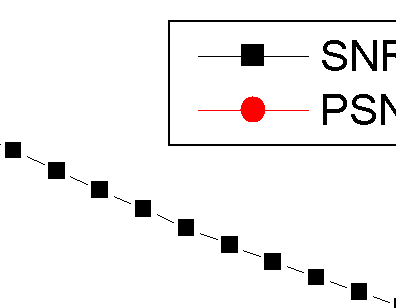
\includegraphics[width=\ww\linewidth]{nazwapliku}}
\hfill% wypełnenie
\subfloat[opis]{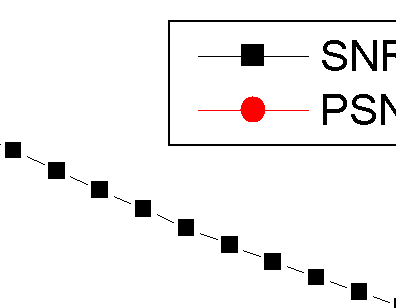
\includegraphics[width=\ww\linewidth]{nazwapliku}}
\hfill%
\subfloat[opis]{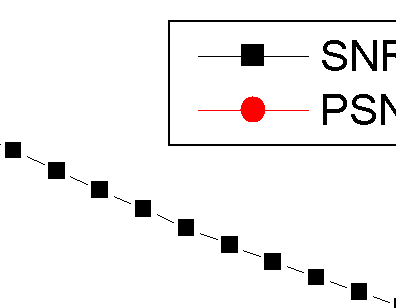
\includegraphics[width=\ww\linewidth]{nazwapliku}}
\hfill%
\subfloat[opis]{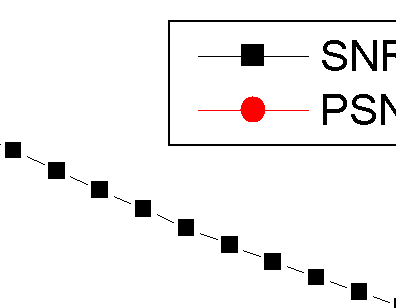
\includegraphics[width=\ww\linewidth]{nazwapliku}}
\caption{Podpis całej ilustracji} %
\end{figure}

\renewcommand{\ww}{0.3}


\begin{figure}
%
\captionsetup[subfloat]{position=bottom,labelformat=empty} %
\subfloat[aaaa][BMP: size=x1~kB; PNG: PSNR=INF, size=x2~kB]{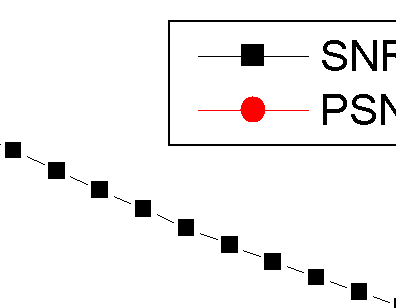
\includegraphics[width=\ww\linewidth]{obraz1}}
\hfill%
\subfloat[GIF: PSNR=x1~dB, size=x2~kB]{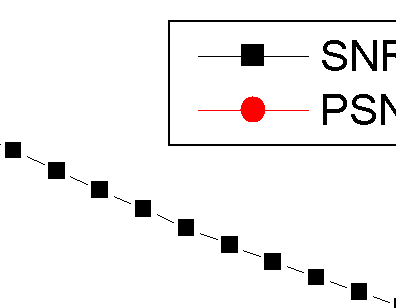
\includegraphics[width=\ww\linewidth]{obraz1_gif}}
\hfill% wypełnenie
\subfloat[opis]{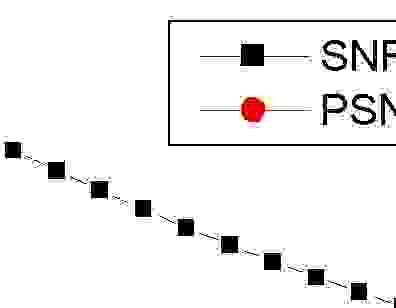
\includegraphics[width=\ww\linewidth]{obraz1_q=1.jpg}}\\ %nowa linia
\subfloat[opis]{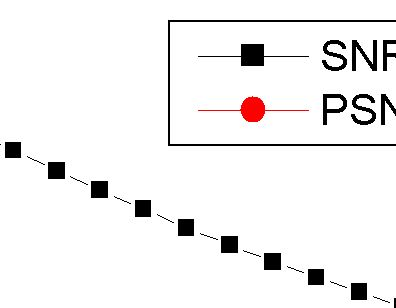
\includegraphics[width=\ww\linewidth]{obraz1_q=80.jpg}}
\hfill%
\subfloat[][JP2: Q=8, PSNR=x dB, size=s kB]{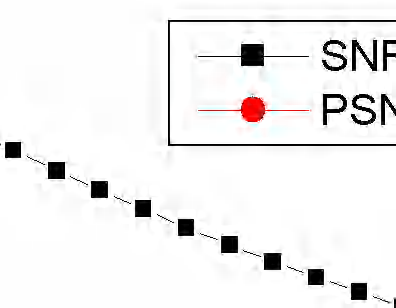
\includegraphics[width=\ww\linewidth]{obraz1_Q=8_jp2}}
\hfill%
\subfloat[opis]{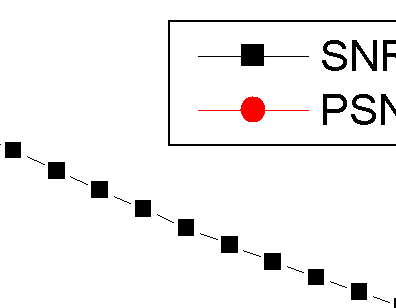
\includegraphics[width=\ww\linewidth]{obraz1_Q=30_jp2}}
\caption{Podpis całej ilustracji} %
\end{figure}

\end{document}